\documentclass[a4paper,14pt]{article}

\usepackage{comment} % Para comentar várias linhas ao mesmo tempo

%matemática
\usepackage{amsmath}
\usepackage{amssymb}

%diagramação
\usepackage{extsizes}
\everymath{\displaystyle}
\usepackage{geometry}
\usepackage{fancyhdr}
\usepackage{multicol}
\usepackage{graphicx}
\usepackage[brazil]{babel}
\usepackage[shortlabels]{enumitem}
\usepackage{cancel}
\usepackage{textcomp}
\usepackage{tcolorbox}

%tabelas
\usepackage{array} % Para melhor formatação de tabelas
\usepackage{longtable}
\usepackage{booktabs}  % Para linhas horizontais mais bonitas
\usepackage{float}   % Para usar o modificador [H]
\usepackage{caption} % Para usar legendas em tabelas
\usepackage{wrapfig} % Para usar tabelas e figuras flutuantes
\usepackage{xcolor} % Para cores do fundo de tabelas
\usepackage{colortbl} % Para cores do fundo de tabelas
\usepackage{upgreek} % Para inserir caracteres gregos

%tikzpicture
\begin{comment}
	\usepackage{tikz}
	\usepackage{scalerel}
	\usepackage{pict2e}
	\usepackage{tkz-euclide}
	\usetikzlibrary{calc}
	\usetikzlibrary{patterns,arrows.meta}
	\usetikzlibrary{shadows}
	\usetikzlibrary{external}
\end{comment}


%pgfplots
\usepackage{pgfplots}
\pgfplotsset{compat=newest}
\usepgfplotslibrary{statistics}
\usepgfplotslibrary{fillbetween}

%colours
\usepackage{xcolor}



\columnsep=2cm
\hoffset=0cm
\textwidth=8cm
\setlength{\columnseprule}{.1pt}
\setlength{\columnsep}{2cm}
\renewcommand{\headrulewidth}{0pt}
\geometry{top=1in, bottom=1in, left=0.7in, right=0.5in}

\pagestyle{fancy}
\fancyhf{}
\fancyfoot[C]{\thepage}

\begin{document}
	
	\noindent\textbf{6FMA145 - Matemática} 
	
	\begin{center}Razão de semelhança (Versão estudante)
	\end{center}
	
	\noindent\textbf{Nome:} \underline{\hspace{10cm}}
	\noindent\textbf{Data:} \underline{\hspace{4cm}}
	
	%\section*{Questões de Matemática}
	
	\begin{multicols}{2}
	    \noindent Sabendo que $\Delta$$ABC \sim \Delta$$A'B'C'$, temos que a razão de semelhança $k$, do primeiro triângulo para o segundo, é dada por: \\\\
	    $k = \frac{AB}{A'B'} = \frac{BC}{B'C'} = \frac{AC}{A'C'}$
		\noindent\textsubscript{--------------------------------------------------------------------------}
		\begin{enumerate} 
			\item Ao quadruplicar as medidas dos lados de um triângulo obtemos um triângulo semelhante. Qual é a razão de semelhança? \\\\\\\\\\\\\\\\\\\\
			\item O triângulo $ABC$ é semelhante ao triângulo $DEF$. Sabe-se que $AB = 3,7DE$. Qual é a razão de semelhança? \\\\\\\\\\\\\\\\\\
			\item Foi feita uma ampliação de 25\% de uma figura. Qual é a razão de semelhança entre o original e a cópia? \\\\\\\\\\\\\\\\\\\\
			\item Sabe-se que $\Delta$$PQR \sim \Delta$$EFG$, sendo $EF = 10, FG = 24$ e $EG = 26$. Calcule as dimensões do triângulo $PQR$ nos seguintes casos, nos quais $k$ é a razão de semelhança entre os triângulos $PQR$ e $EFG$:
			\begin{enumerate}[a)]
				\item $k = \frac{1}{2}$ \\\\\\\\\\\\\\\\
				\item $k = 3,7$ \newpage
				\item $k = \frac{7}{9}$ \\\\\\\\\\\\\\\\
			\end{enumerate}
			\textbf{Desafio olímpico} \\\\
			No retângulo $ABCD$ abaixo, Júlia traçou algumas retas e criou os ângulos de 18°, $\uptheta$, 29° e 13°. Qual é o valor de $\uptheta$? \\
			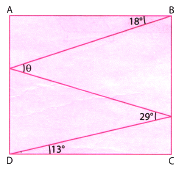
\includegraphics[width=1\linewidth]{6FMA145_imagens/imagem1}
			\begin{enumerate}[a)]
				\item 21°
				\item 34°
				\item 42°
				\item 47°
				\item 50° \\\\\\\\\\\\\\
			\end{enumerate}
			% 88 a 90
			\item Ao reduzir a um quinto as medidas dos lados de um triângulo, obtemos outro triângulo, semelhante ao primeiro. Qual é a razão de semelhança? \\\\\\\\\\\\\\\\\\\\
			\item Foi tirada cópia de uma foto, com redução de 60\%. Qual é a razão de semelhança entre o original e a cópia? \\\\\\\\\\\\\\\\\\\\
		\end{enumerate}
			 $~$ \\ $~$ \\ $~$ \\ $~$ \\ $~$ \\ $~$ \\ $~$ \\ $~$ \\ $~$ \\ $~$ \\ $~$ \\
	\end{multicols}
\end{document}